%--------------Preamble----------------------------------------------------
%\documentclass[aspectratio=1610,10pt,ucs]{beamer} % K1520
%\documentclass[aspectratio=169,10pt,ucs]{beamer} % alle anderen
\documentclass[aspectratio=43,10pt,ucs]{beamer} % safe workaround
%\documentclass[handout,10pt,ucs]{beamer} % for creating handouts
%-------------------------------------------------------------------------

%%
%% definition of perlis mathclap etcpp.
%%

% For comparison, the existing overlap macros:
% \def\llap#1{\hbox to 0pt{\hss#1}}
% \def\rlap#1{\hbox to 0pt{#1\hss}}
\def\clap#1{\hbox to 0pt{\hss#1\hss}}
\def\mathllap{\mathpalette\mathllapinternal}
\def\mathrlap{\mathpalette\mathrlapinternal}
\def\mathclap{\mathpalette\mathclapinternal}
\def\mathllapinternal#1#2{%
  \llap{$\mathsurround=0pt#1{#2}$}}
\def\mathrlapinternal#1#2{%
  \rlap{$\mathsurround=0pt#1{#2}$}}
\def\mathclapinternal#1#2{%
  \clap{$\mathsurround=0pt#1{#2}$}}

%%
%% end of perlis stuff
%%

%% hack for amsmath pmatrix and similar
\makeatletter
\renewcommand*\env@matrix[1][*\c@MaxMatrixCols c]{%
  \hskip -\arraycolsep
  \let\@ifnextchar\new@ifnextchar
  \array{#1}}
\makeatother

\newcommand{\backupbegin}{
   \newcounter{framenumberappendix}
   \setcounter{framenumberappendix}{\value{framenumber}}
}
\newcommand{\backupend}{
   \addtocounter{framenumberappendix}{-\value{framenumber}}
   \addtocounter{framenumber}{\value{framenumberappendix}} 
}
%%%%% bold letters
\newcommand{\bfA}{{\mathbf A}}
\newcommand{\bfB}{{\mathbf B}}
\newcommand{\bfC}{{\mathbf C}}
\newcommand{\bfD}{{\mathbf D}}
\newcommand{\bfE}{{\mathbf E}}
\newcommand{\bfF}{{\mathbf F}}
\newcommand{\bfG}{{\mathbf G}}
\newcommand{\bfH}{{\mathbf H}}
\newcommand{\bfI}{{\mathbf I}}
\newcommand{\bfJ}{{\mathbf J}}
\newcommand{\bfK}{{\mathbf K}}
\newcommand{\bfL}{{\mathbf L}}
\newcommand{\bfM}{{\mathbf M}}
\newcommand{\bfN}{{\mathbf N}}
\newcommand{\bfO}{{\mathbf O}}
\newcommand{\bfP}{{\mathbf P}}
\newcommand{\bfQ}{{\mathbf Q}}
\newcommand{\bfR}{{\mathbf R}}
\newcommand{\bfS}{{\mathbf S}}
\newcommand{\bfT}{{\mathbf T}}
\newcommand{\bfU}{{\mathbf U}}
\newcommand{\bfV}{{\mathbf V}}
\newcommand{\bfW}{{\mathbf W}}
\newcommand{\bfX}{{\mathbf X}}
\newcommand{\bfY}{{\mathbf Y}}
\newcommand{\bfZ}{{\mathbf Z}}
\newcommand{\bfa}{{\mathbf a}}
\newcommand{\bfb}{{\mathbf b}}
\newcommand{\bfc}{{\mathbf c}}
\newcommand{\bfd}{{\mathbf d}}
\newcommand{\bfe}{{\mathbf e}}
\newcommand{\bff}{{\mathbf f}}
\newcommand{\bfg}{{\mathbf g}}
\newcommand{\bfh}{{\mathbf h}}
\newcommand{\bfi}{{\mathbf i}}
\newcommand{\bfj}{{\mathbf j}}
\newcommand{\bfk}{{\mathbf k}}
\newcommand{\bfl}{{\mathbf l}}
\newcommand{\bfm}{{\mathbf m}}
\newcommand{\bfn}{{\mathbf n}}
\newcommand{\bfo}{{\mathbf o}}
\newcommand{\bfp}{{\mathbf p}}
\newcommand{\bfq}{{\mathbf q}}
\newcommand{\bfr}{{\mathbf r}}
\newcommand{\bfs}{{\mathbf s}}
\newcommand{\bft}{{\mathbf t}}
\newcommand{\bfu}{{\mathbf u}}
\newcommand{\bfv}{{\mathbf v}}
\newcommand{\bfw}{{\mathbf w}}
\newcommand{\bfx}{{\mathbf x}}
\newcommand{\bfy}{{\mathbf y}}
\newcommand{\bfz}{{\mathbf z}}

%% extra bold symbols
\newcommand{\bfell}{{\boldsymbol{\ell}}}
\newcommand{\bfLambda}{{\boldsymbol{\Lambda}}}
\newcommand{\bfSigma}{{\boldsymbol{\Sigma}}}
\newcommand{\bfnu}{{\boldsymbol{\nu}}}
\newcommand{\bfphi}{{\boldsymbol{\phi}}}
\newcommand{\bfalpha}{{\boldsymbol{\alpha}}}
\newcommand{\bfbeta}{{\boldsymbol{\beta}}}
\newcommand{\bfhatbeta}{{\boldsymbol{\widehat{\beta}}}}
\newcommand{\bfomega}{{\boldsymbol{\omega}}}
\newcommand{\bfrho}{{\boldsymbol{\rho}}}
\newcommand{\bfmu}{{\boldsymbol{\mu}}}
\newcommand{\bfchecknu}{{\boldsymbol{\check{\nu}}}}
\newcommand{\bfhatnu}{{\boldsymbol{\widehat{\nu}}}}

%% new /renewed commands
\newcommand{\Span}{\mathop{\mathsf{span}}}
\renewcommand{\deg}{\mathop{\mathsf{deg}}}
\renewcommand{\min}{\mathop{\mathsf{min}}}
\newcommand{\argmin}{\mathop{\mathsf{argmin}}}
\renewcommand{\max}{\mathop{\mathsf{max}}}
\newcommand{\spec}{\mathop{\mathsf{spec}}}
\newcommand{\ucup}{\ensuremath{\mathop{\cup}\limits}}

\mode<presentation>
{
  \usetheme{ABMATH}
  \useinnertheme{default}
  \setbeamercovered{invisible}
  \setbeamertemplate{navigation symbols}{} % supress all navigation symbols
  \usefonttheme[onlymath]{serif}
  \setbeamertemplate{items}[triangle]
  \setbeamertemplate{sections/subsections in toc}[default]
  \setbeamertemplate{enumerate items}[circle]
}

\usepackage[utf8x]{inputenc}
\usepackage[T1]{fontenc}
\PreloadUnicodePage{32} % for „ and “
\usepackage[russian,german,english]{babel}
\usepackage{graphicx}
\usepackage{times}
\usepackage{pifont}
%%%% begin - for shaded boxes around equations
\usepackage{empheq} % brauche ich hier nicht
\usepackage[many]{tcolorbox}
\newtcbox{\mybox}[1][]{nobeforeafter,math upper,tcbox raise base,
  enhanced,frame hidden,boxrule=0pt,interior style={top color=magenta!10!red,
  bottom color=magenta!10!red,middle color=magenta!30!white},
  fuzzy halo=1pt with magenta,drop large lifted shadow,#1}
%%%% end - for shaded boxes around equations
\usepackage{ulem}
\normalem
\newcommand{\soutb}[3]{%
  \only<#1>{{#3}}%
  \uncover<#2>{\textcolor{black!30!}{\sout{#3}}}}
%%%
\hypersetup{%
  pdftitle     = {How to give a good talk},
  pdfsubject   = {YRM 2018 at Plön},
  pdfkeywords  = {YRM 2018, good talk},
  pdfauthor    = {\textcopyright\ Jens-Peter M. Zemke 2018},
%  pdfpagemode  = FullScreen
}

\title{How to give a good talk}
\subtitle{Adapted from a talk by Simon Peyton Jones/Microsoft and
  notes by Tamara Kolda \& Virginia Torczon/SIAM News}

\author[Jens-Peter M. Zemke]{%
  Jens-Peter M. Zemke}

\institute{\href{http://www.tu-harburg.de/mat/}{%
              Institut für Mathematik}\\
            Lehrstuhl Numerische Mathematik\\
           \href{http://www.tu-harburg.de/}{%
            Technische Universität Hamburg}}

\date{27.03.2018}

\titlegraphic{%
%  \vspace*{-1.5em} % if date is empty
  \includegraphics[height=.15\textheight]%
%    {pics/MATH_de}% %%% German
    {pics/MATH_en}% %%% English
  \hspace*{.2\textwidth}
  \includegraphics[height=.15\textheight]%
%    {pics/TUHH_de}% %%% German
    {pics/TUHH_en}% %%% English
}

%Delete this, if you do not want the table of contents to pop up at
%the beginning of each section:
\AtBeginSection[]
{
  \begin{frame}<beamer>
    \frametitle{Overview}
    \tableofcontents[currentsection]
  \end{frame}
}
%---------------------------preamble-----------------------------------
\begin{document}
%----------------------------begin frame-------------------------------
\begin{frame}
  \titlepage
\end{frame}
%----------------------------end frame---------------------------------
%\usebackgroundtemplate{%
%  \includegraphics[width=\paperwidth]{pics/Background}}
%----------------------------begin frame-------------------------------
\begin{frame}
  \frametitle{Why you should listen to this talk}

  \textcolor{blue}{Research is communication}

  \vspace*{1em}

  \begin{itemize}
  \item Everyone has to give talks, but how often do you
    \textcolor{blue}{enjoy} talks by others? Your own?
  \item Some \textcolor{blue}{simple, actionable ideas} that can make
    your talks much better
  \item You will have \textcolor{blue}{more fun}
  \item A talk gives you \textcolor{blue}{access to the world's most
      priceless commodity}: the time and attention of other
    people. \alert{Don't waste it!}
  \end{itemize}

  \uncover<2->{%
  \vspace*{3em}
  \hfill As seen here $\leadsto$ start with a motiviation!}

\end{frame}
%----------------------------end frame---------------------------------
%----------------------------begin frame-------------------------------
\begin{frame}
  \frametitle{Overview
      \uncover<2->{\alert{(possibly omit the overview!)}}}
  \tableofcontents
  % You might wish to add the option [pausesections]
\end{frame}
%----------------------------end frame---------------------------------
\section{The setting}
\subsection{Purpose of a talk}
%----------------------------begin frame-------------------------------
\begin{frame}
  \frametitle{Purpose of a talk}

  The purpose of your talk \alert{is not}:
  \begin{itemize}
  \item \alert{To impress} your audience \alert{with your brainpower}
  \item To tell them \alert{everything} you know about the topic
  \item To present all the \alert{technical details}
  \end{itemize}

  \vspace*{1em}

  \uncover<2->{%
  The purpose of your talk \textcolor{blue}{is}:
  \begin{itemize}
  \item To give your audience an \textcolor{blue}{intuitive feel} for
    your idea
  \item To make them foam at the mouth with \textcolor{blue}{eagerness
      to read your paper}
  \item To \textcolor{blue}{engage, excite, provoke} them
  \item To make them \textcolor{blue}{glad they came}
  \end{itemize}}

  % \item \soutb{1-1}{2-}{Supervisor insists}
  % \item \soutb{1-1}{2-}{everybody does}

  \vspace*{1em}

  \uncover<3->{%
  Your paper: \textcolor{blue}{the beef}, your talk:
  \textcolor{blue}{the beef advertisement}\\
  \hfill $\leadsto$ \alert{do not confuse the two!}}

\end{frame}
%----------------------------end frame---------------------------------
\subsection{The key idea, the audience, \& you}
%----------------------------begin frame-------------------------------
\begin{frame}
  \frametitle{Your key idea}

  If the audience remembers only one thing from your talk, what should
  it be?

  \vspace*{1em}

  \begin{itemize}
  \item You \alert{must} identify a key idea.\\
    {\small ``My supervisor wanted me to give a talk'' is No Good.}
  \item Be \textcolor{blue}{specific}.\\
    {\small Don't leave your audience to figure it out for
      themselves. Spoiler: They won't.}
  \item Be absolutely \textcolor{blue}{specific}.\\
    {\small Say: ``If you remember nothing else, remember this.''}
  \item Organise your talk around this \textcolor{blue}{specific}
    goal.\\
    {\small Ruthlessly prune all material that is irrelevant to this
      goal.}
  \end{itemize}

\end{frame}
%----------------------------end frame---------------------------------
%----------------------------begin frame-------------------------------
\begin{frame}
  \frametitle{The audience}

  The audience you \textcolor{blue}{would like}
  \begin{itemize}
  \item Have read all your earlier papers
  \item Thoroughly understand all the relevant theory of
    antiderivations of degree 1 on the exterior algebra of
    differential forms in local coordinates
  \item Are all agog to hear about the latest developments in your
    work
  \item Are fresh, alert and ready for action
  \end{itemize}

  \vspace*{1em}

  \uncover<2->{%
  The audience you \alert{get}
  \begin{itemize}
  \item Have never heard of you
  \item Have heard of exterior algebras, but wish they hadn't
  \item Have just had lunch and are ready for a doze
  \end{itemize}}

  \vspace*{1em}

  \uncover<3->{%
  Your mission is to \textcolor{blue}{WAKE THEM UP} and make them glad
  they did}

\end{frame}
%----------------------------end frame---------------------------------
%----------------------------begin frame-------------------------------
\begin{frame}
  \frametitle{You}

  You are the \alert{filter} between the key idea and the audience.

  \vspace*{1em}

  \uncover<2->{%
  \textcolor{blue}{Enthusiasm!} Your most potent weapon:
  \begin{itemize}
  \item If you do not seem excited by your idea, why should the
    audience be?
  \item Enthusiasm makes people dramatically more receptive
  \item It gets you loosened up, breathing, moving around
  \end{itemize}}

  \vspace*{1em}

  \uncover<3->{%
  \alert{No apologies}.
  \begin{itemize}
  \item ``I didn't have time to prepare this talk properly''
  \item ``My computer broke down, so I don't have the results I
    expected''
  \item ``I don't have time to tell you about this''
  \item ``The dog ate my homework''
  \end{itemize}}

\end{frame}
%----------------------------end frame---------------------------------
%----------------------------begin frame-------------------------------
\begin{frame}
  \frametitle{You}

  You will most probably experience severe \alert{pre-talk symptoms}:
  \begin{itemize}
  \item Inability to breathe
  \item Inability to stand up (legs give way)
  \item Inability to operate brain
  \item Inability to make eye-contact
  \end{itemize}

  \vspace*{1em}

  \uncover<2->{%
  \textcolor{blue}{Countermeasures}:
  \begin{itemize}
  \item Deep breathing during previous talk
  \item Script your first few sentences precisely ($\leadsto$ no brain
    required)
  \item Move around a lot, use large gestures, wave your arms, stand
    on chairs
  \item Go to the loo first
  \item Look at a friendly person in the first row/a point
    20\,cm above the heads
  \end{itemize}}

\end{frame}
%----------------------------end frame---------------------------------
\section{Structure}
\subsection{1: Motivation (20\%)}
%----------------------------begin frame-------------------------------
\begin{frame}
  \frametitle{Motivate your audience}

  \alert{You have 2 minutes} to engage your audience before they start
  to doze.

  \vspace*{1em}

  They are thinking \ldots
  \begin{itemize}
  \item Why should I tune into this talk?
  \item What is the problem? (Hopefully not the talk.)
  \item Why is it an interesting problem?
  \item Does this talk describe a worthwhile advance?
  \end{itemize}

  \vspace*{2em}

  \uncover<2->{%
  \textcolor{blue}{Don't waste your two minutes!}}

  \vspace*{1em}

  \uncover<2->{%
  \textcolor{tuhh_cyan}{Example:} Solving linear systems is a building
  block in the inner loop of every optimization routine. By solving
  them faster you can increase the speed of your topological
  optimization by a factor of 10--30, as I will show you.}

\end{frame}
%----------------------------end frame---------------------------------
\subsection{2: Your key idea (70\%-80\%)}
%----------------------------begin frame-------------------------------
\begin{frame}
  \frametitle{\{Narrow, deep\} beats \{wide, shallow\}}

  \vspace*{1em}

  \uncover<1>{%
  \begin{itemize}
  \item \textcolor{blue}{Avoid shallow overviews at all costs}
  \item Cut to the chase: the technical ``meat''
  \item It's ok to cover only part of your paper/work
  \end{itemize}}

  \vspace*{-2em}

  \begin{center}
    
\includegraphics[width=\textwidth,%
    height=.7\textheight%,clip,trim=0mm 0mm 52mm 31mm
    ]{pics/soil-loch}
  \end{center}\vspace*{-1.2em}
  {\tiny \hfill Pixabay/OpenClipart-Vectors}

  \uncover<2->{%
  \begin{tikzpicture}[remember picture,overlay,-stealth]
    \path[blue,line width=0.2cm](2,8.7)edge[bend left](3.6,2);
    \node[blue] at (2.3,7) {Good!};
    \path[red,line width=0.2cm](6.5,8.7)edge[bend right](9,5.7);
    \node[red] at (8,7) {Bad.};
  \end{tikzpicture}}

\end{frame}
%----------------------------end frame---------------------------------
%----------------------------begin frame-------------------------------
\begin{frame}
  \frametitle{Examples are your main weapon}

  \textcolor{blue}{Omit rather the general case, not the example.}

  \vspace*{.5em}

  \alert{Examples}
  \begin{itemize}
  \item To motivate the work
  \item To convey the basis intuition
  \item To illustrate Your Idea in action
  \item To show extreme cases
  \item To highlight shortcomings
  \end{itemize}

  \vspace*{.5em}

  \uncover<2->{%
  Convergence \textcolor{blue}{graphs} carry much more information
  than \alert{tables} with values!

  \vspace*{-.5em}

  \begin{columns}
    \begin{column}{.5\textwidth}
      \begin{center}
        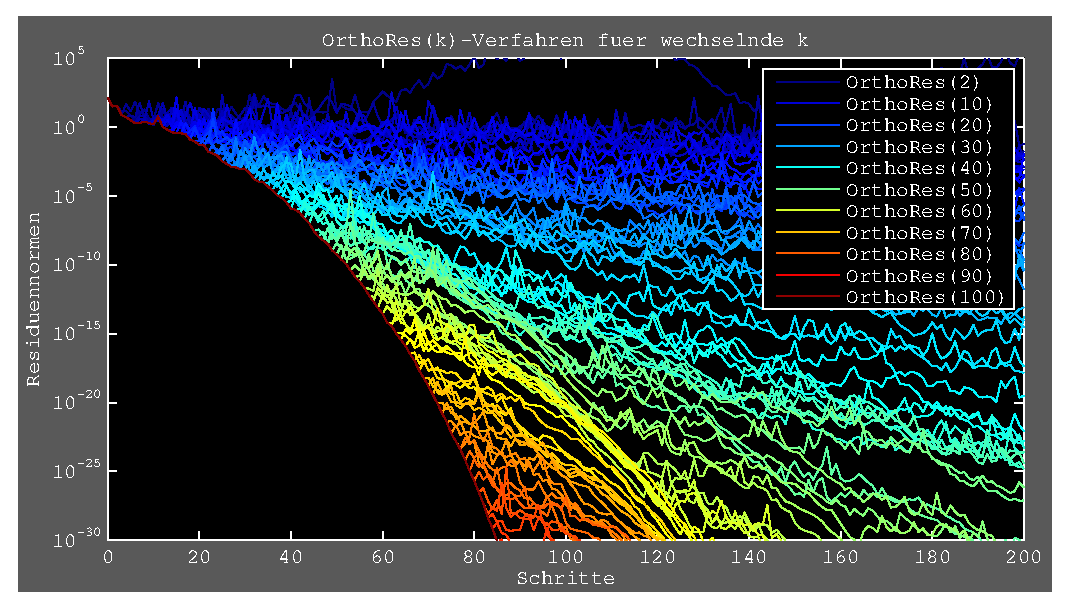
\includegraphics[width=\textwidth]{pics/OrthoResK}
      \end{center}
    \end{column}
    \begin{column}{.4\textwidth}
      \begin{center}
        \begin{tabular}{cccc}
          $k$ \textbackslash\ $m$ & $120$ & $140$ & $160$ \\\hline
          $10$ & $\star$ & $\star$ & $\star$ \\
          $20$ & $\star$ & $\star$ & $\star$ \\
          $30$ & $\star$ & $\star$ & $\star$ \\
          $40$ & $\star$ & $\star$ & $\star$ \\
          $50$ & $\star$ & $\star$ & $\star$ \\
          $60$ & $\star$ & $\star$ & $\star$ \\
        \end{tabular}
      \end{center}
    \end{column}
  \end{columns}}

\end{frame}
%----------------------------end frame---------------------------------
%----------------------------begin frame-------------------------------
\begin{frame}
  \frametitle{What to leave out}

  \alert{Outline} of my talk:

  \begin{columns}
    \begin{column}[t]{.5\textwidth}
      \begin{itemize}
      \item Motivation
      \item Introduction
      \item The method
      \item Numerical examples
      \item Conclusions \& Outlook
      \end{itemize}

      \vspace*{1em}

      \uncover<3->{A \textcolor{blue}{motivation} is better than
        \begin{itemize}
        \item A standard outline
        \item An outline for experts (i.e., mostly only the speaker
          him-/herself)
        \end{itemize}
      }

      \vspace*{1em}

      \uncover<4->{But: The outline can be the motivation.}
    \end{column}
    \begin{column}[t]{.5\textwidth}
    \uncover<2->{%
      \begin{itemize}
      \item Background
      \item The PAMDD system
      \item Shortcomings of PAMDD
      \item Overview of real-harmonic polynomials
      \item The Betti numbers of the weak-* transitive co-diffable
        Sherkovski ideal in PAMDD
      \item Benchmarks
      \item Related work
      \item Conclusions and further work
      \item References
      \end{itemize}}
    \end{column}
  \end{columns}

  \uncover<2->{%
  \begin{tikzpicture}[overlay,-stealth]
    \draw[-,red,thick,line width=.2cm,opacity=0.6]
      (0.5,5.7)--(3.5,3.5);
  \end{tikzpicture}}

  \uncover<3->{%
  \begin{tikzpicture}[overlay,-stealth]
    \draw[-,red,thick,line width=.2cm,opacity=0.6]
      (6.8,6.2)--(11,.5);
  \end{tikzpicture}}

\end{frame}
%----------------------------end frame---------------------------------
%----------------------------begin frame-------------------------------
\begin{frame}
  \frametitle{What to leave out}

  Concerning the \alert{outline}:
  \begin{description}
  \item[$\boldsymbol{-}$] Conveys near zero information at the start
    of your talk
  \item[$\boldsymbol{-}$] Since your audience only gives you 2 minutes
    before dozing, you've just lost them
  \item[$\boldsymbol{+}$] Maybe put up an outline for orientation
    after your motivation
  \item[$\boldsymbol{+}$] \ldots and signposts at pause points during
    the talk
  \end{description}

  \vspace*{2em}

  \uncover<2->{%
  Leave out \alert{related work}, but:
  \begin{itemize}
  \item You absolutely must \textcolor{blue}{know the related work},
    respond readily to questions
  \item \textcolor{blue}{Acknowledge co-authors} (title slide) and
    pre-cursors
  \item ``X's very interesting work does Y; I have extended it to Z''
  \end{itemize}}

\end{frame}
%----------------------------end frame---------------------------------
%----------------------------begin frame-------------------------------
\begin{frame}
  \frametitle{What to leave out}

  Leave out \alert{technical detail/detailed formulas}:
  {\tiny
  \[
    \bfT_5 =
    \begin{pmatrix}
      \frac{11}{10} & \frac{\sqrt{193}\,\sqrt{200}}{200} & 0 & 0 & 0\\
      \frac{\sqrt{193}\,\sqrt{200}}{200} & \frac{4517}{1930} &
        \frac{\sqrt{199955}}{772} & 0 & 0\\
      0 & \frac{\sqrt{199955}}{772} & \frac{1688137}{2205218} &
        \frac{\sqrt{48641211}\,\sqrt{913874332}}{913874332} & 0\\
      0 & 0 & \frac{\sqrt{48641211}\,\sqrt{913874332}}{913874332} &
      \frac{103198117}{159981139} &
        \frac{\sqrt{155536425}\,\sqrt{5489176063}}{5489176063}\\
      0 & 0 & 0 &
      \frac{\sqrt{155536425}\,\sqrt{5489176063}}{5489176063} &
      \frac{18174}{28003}
    \end{pmatrix}
  \]}
  Better: $\bfT_5$ is unreduced symmetric tridiagonal.

  \vspace*{1em}

  \uncover<2->{%
  \begin{itemize}
  \item Even though every line is drenched in your blood and sweat,
    \textcolor{blue}{dense clouds of notation will send your audience
      immediatly to sleep}
  \item Present specific aspects only; \textcolor{blue}{refer to the
      paper} for details
  \item By all means have backup slides to use in response to
    questions
  \end{itemize}}

\end{frame}
%----------------------------end frame---------------------------------
\subsection{3: Conclusions or bust (0\%-10\%)}
%----------------------------begin frame-------------------------------
\begin{frame}
  \frametitle{Do we need conclusions?}

  Simon Peyton Jones: \alert{There is no 3.}

  \vspace*{3em}

  \uncover<2->{%
  Use the \textcolor{blue}{conclusions as last slide}, no ``Thank
  you!''
  \begin{itemize}
  \item Sketch main message on last slide
  \item Summarize most important aspects
  \item Good basis for discussion/questions
  \item Try to fit \alert{everything on one slide}
  \end{itemize}}

\end{frame}
%----------------------------end frame---------------------------------
\section{Preparing your slides}
%----------------------------begin frame-------------------------------
\begin{frame}
  \frametitle{Write your slides …}

  \begin{description}
  \item[Simon Peyton Jones:] the night before (or at least, polish it
    then)
  \item[Tamara Kolda \& Virginia Torczon:] An $m$-minute talk to $n$
    people \alert{will consume $mn$ person-minutes}. It's only
    courteous to put at least that much time into preparing the talk!
  \end{description}

  \vspace*{1em}

  \uncover<2->{%
  But:
  \begin{itemize}
  \item Your talk absolutely must be fresh on your mind!
  \item Ideas will occur to you during the conference, as you obsess
    on your talk during other people's presentations
  \item You may learn that some of your assumptions are outdated or
    obsolete
  \end{itemize}

  \vspace*{1em}

  \textcolor{blue}{Best to finalize/polish the slides the night/minute
    before the talk}}

\end{frame}
%----------------------------end frame---------------------------------
%----------------------------begin frame-------------------------------
\begin{frame}
  \frametitle{Don't limit your color scheme unecessarily}

  \begin{itemize}
  \item Mathematical talks \textcolor{blue}{have evolved} from white
    on black/black on white
  \item The use of \textcolor{blue}{colors} always makes slides
    \textcolor{blue}{more interesting}
  \item Introduced thoughtfully, color clearly
    \textcolor{blue}{emphasizes} key ideas and
    \textcolor{blue}{establishes connections} between related concepts
  \end{itemize}

  \vspace*{3em}
  
  (\#9 in ``Top Ten Ways to Lose an Audience'' by Tamara Kolda/Virginia
   Torczon)

\end{frame}
%----------------------------end frame---------------------------------
%----------------------------begin frame-------------------------------
\begin{frame}
  \frametitle{Balance your layout}

  \begin{itemize}
  \item Choose fonts of \alert{sufficient size} and in a
    \textcolor{blue}{clean, simple typeface}
  \item Don't use complete sentences from your paper, rewrite into
    short, \textcolor{blue}{crispy notes}
  \item Don't simply copy graphics from your paper, \alert{increase
      font size} of labels, legend and \alert{thickness of lines}
  \item Just \alert{refrain from yellow and (light) green on white},
    especially in graphs
  \item Test your talk in a room of similar size than the one your are
    speaking in from the background for readability, invisible colors
    and lines that are too thin, \textcolor{blue}{go back and fix
      them!}
  \end{itemize}
  
  \vspace*{1em}
  
  (\#8, \#7 in ``Top Ten Ways to Lose an Audience'' by Tamara
   Kolda/Virginia Torczon)

\end{frame}
%----------------------------end frame---------------------------------
%----------------------------begin frame-------------------------------
\begin{frame}
  \frametitle{Minimize acronyms and math symbols}

  \begin{itemize}
  \item Listeners will only \textcolor{blue}{remember a few
      new-to-them concepts across slides}
  \item A talk is not a paper where you can add a section on notation
  \item You do get \textcolor{blue}{``standard'' notation for free},
    but be careful: numerical linear algebra: $\bfA\bfx=\bfb$, mechanics:
    $\bfK\bfu=\bff$, stochastics: $\bfX\beta=\bfy$.
  \item \alert{Repeat important formulae/definitions} where needed!
  \end{itemize}

  \vspace*{3em}
  
  (\#6 in ``Top Ten Ways to Lose an Audience'' by Tamara
   Kolda/Virginia Torczon)

\end{frame}
%----------------------------end frame---------------------------------
%----------------------------begin frame-------------------------------
\begin{frame}
  \frametitle{Context / Background}

  \begin{itemize}
  \item \alert{Put your work into context!} The audience (typically)
    does not comprise the experts in the field.
  \item Work out the \textcolor{blue}{importance of your
      contribution}: What has changed?
  \item For the experts in the audience: stress \textcolor{blue}{how
      your work fits in the broader context} of the field
  \item Give \alert{enough background to be understandable}, yet leave
    room for your contribution
  \item Few things are more boring than sitting through a review of
    material you've seen a dozen times before
  \end{itemize}

  \vspace*{1em}

  (\#5, \#4 in ``Top Ten Ways to Lose an Audience'' by Tamara
   Kolda/Virginia Torczon)

\end{frame}
%----------------------------end frame---------------------------------
\section{Presenting your talk}
%----------------------------begin frame-------------------------------
\begin{frame}
  \frametitle{Being …}

  \alert{Being seen:}
  \begin{itemize}
  \item \textcolor{blue}{Face the audience}, not the screen
  \item \textcolor{blue}{Know your material}
  \item Put your laptop in front of you, \textcolor{blue}{screen
      towards you}
  \item \textcolor{blue}{Don't point much}, but when you do, point at
    the projection, not at your laptop
  \item When pointing with a laser pointer, circle to hide trembling
    hands
  \end{itemize}

  \vspace*{1em}

  \uncover<2->{%
  \alert{Being heard:}
  \begin{itemize}
  \item \textcolor{blue}{Speak to someone at the back of the room},
    even if you have a microphone on
  \item \textcolor{blue}{Make eye contact}; identify a nodder and
    speak to her or him (better still, more than one)
  \item \textcolor{blue}{Watch audience} for questions …
  \end{itemize}}

\end{frame}
%----------------------------end frame---------------------------------
%----------------------------begin frame-------------------------------
\begin{frame}
  \frametitle{Questions/Finishing}

  \alert{Questions?}
  \begin{itemize}
  \item Questions are \textcolor{blue}{not a problem}
  \item Questions are \textcolor{blue}{a golden$^3$ opportunity} to
    connect with your audience
  \item Specifically \textcolor{blue}{encourage questions} during your
    talk: pause briefly now and then, ask for questions
  \end{itemize}

  \vspace*{1em}

  \uncover<2->{%
  \alert{Finishing.}
  \begin{itemize}
  \item Absolutely without fail, \alert{finish on time}
  \item Audiences get restive and \textcolor{blue}{essentially stop
      listening} when your time is up
  \item \textcolor{blue}{Simply truncate and conclude}
  \item Do not say ``would you like me to go on?'' (it's hard to say
    ``no thanks'')
  \item Finish on time \alert{even} when all other speakers in your
    session failed to
  \item „Sie können über alles reden, nur nicht über 30 Minuten.“
  \end{itemize}}

\end{frame}
%----------------------------end frame---------------------------------
%----------------------------begin frame-------------------------------
\begin{frame}
  \frametitle{Presenting your slides}

  \begin{itemize}
  \item Use a \textcolor{blue}{wireless presenter gizmo}
  \item \alert{Test} that the laptop works with the projector, in
    advance
  \item Laptops break: leave a \textcolor{blue}{backup copy} on the
    web; bring a \textcolor{blue}{backup copy} on USB flash
  \end{itemize}

  \vspace*{1em}

  \begin{itemize}[<+->]
  \item A very annoying technique
  \item is to reveal
  \item your points
  \item one
  \item by one
  \item by one
  \item by one, unless …
  \item there is a \alert{punch line}
  \end{itemize}

\end{frame}
%----------------------------end frame---------------------------------
%----------------------------begin frame-------------------------------
\begin{frame}
  \frametitle{Presenting your slides}
%                  Horizontal blinds pulled away
%\transblindshorizontal
%                   Vertical blinds pulled away
%\transblindsvertical
%                   Move to center from all sides
%       \transboxin
%                   Move to all sides from center
%      \transboxout
%                   Slowly dissolve what was shown before
\transdissolve<1>
%                   Glitter sweeps in specified direction
%\transglitter
%                   Sweeps two vertical lines in
%\transsplitverticalin
%                   Sweeps two vertical lines out
%\transsplitverticalout
%                   Sweeps two horizontal lines in
%\transhorizontalin
%                   Sweeps two horizontal lines out
%\transhorizontalout
%                   Sweeps single line in specified direction
%\transwipe
%                   Show slide specified number of seconds
%\transduration{2}
%New for PDF 1.5:
%\transcover    % does not work
%\transfade     % ???
%\transpush     % does not work
%\transuncover  % does not work

  Use animation effects\\
  \uncover<1->{\hspace*{4em}very}
  \uncover<1->{\hspace*{12em}very}
  \uncover<1->{\hspace*{2em}very}\\
  \uncover<1->{\hspace*{7em}very}
  \uncover<1->{\hspace*{4em}very}
  \uncover<1->{\hspace*{13em}very}\\
  \uncover<1->{sparingly.}

  \vspace*{1em}

  \uncover<2->{%
    Good papers and talks are a \textcolor{blue}{fundamental part of
      research excellence}
    \begin{itemize}
    \item Invest time
    \item Learn skills
    \item Practice
    \end{itemize}}

  \vspace*{1em}

  \uncover<3->{%
    \textcolor{blue}{Research is communication}, your papers and talks
    \begin{itemize}
    \item \alert{Crystalise your ideas}
    \item \alert{Communicate} them to others
    \item Get \alert{feedback}
    \item Build \alert{relationships}
    \end{itemize}}

\end{frame}
%----------------------------end frame---------------------------------
%----------------------------begin frame------------------------------
\begin{frame}
  \frametitle{Helping and learning from others}

  \textcolor{blue}{Being a good audience member:}
  \begin{itemize}
  \item Eye contact with speaker
  \item Nod frequently
  \item Ask questions:
    \begin{itemize}
    \item Start asking questions when you lose contact with the
      talk. The rest of the audience will thank you for it.
    \item Stop when you sense that you are beginning to de-rail the
      entire talk.
    \end{itemize}
  \end{itemize}

  \vspace*{3em}

  \uncover<2->{%
  You will attend 20-50 times as many talks as you give. Watch others
  people's talks intelligently and \textcolor{blue}{pick up ideas} for
  what to do and what to avoid.

  \vspace*{1em}

  The general standard is often low. \alert{You don't have to be
    outstanding to stand out.}}

\end{frame}
%----------------------------end frame---------------------------------
\section{Beyond the talk: publication}
%----------------------------begin frame------------------------------
\begin{frame}
  \frametitle{Your talk went well? Publish a paper!}

  In the mathematical community a paper
  \begin{itemize}[<+->]
  \item is sent to the \textcolor{blue}{editor-in-chief} of a journal
    w/ \alert{accompanying letter}
  \item based on the \alert{letter, title, and abstract}, an
    \textcolor{blue}{editor} is chosen
  \item based on the \alert{letter, title, and abstract}, the
    \textcolor{blue}{editor} sends your paper to 2--3
    \textcolor{blue}{referees}
  \item the \textcolor{blue}{referees} write referee reports
  \item the \textcolor{blue}{editor} makes a decision based on the
    reports
  \end{itemize}

  \vspace*{1em}

  All this is mostly based on \textcolor{blue}{voluntary work!}

\end{frame}
%----------------------------end frame--------------------------------
\appendix
\backupbegin
%----------------------------begin frame------------------------------
\begin{frame}
  \frametitle{References}
  
  \begin{thebibliography}{}
  \bibitem[Kolda and Torczon, 2011]{KoldaTorczon:2011}
    Tamara Kolda \& Virginia Torczon
    \newblock \emph{Top Ten Ways to Lose an Audience}.
    \newblock SIAM News, Volume 44, Number 3, April 2011.
    \newblock \url{https://www.siam.org/pdf/news/1876.pdf}

  \bibitem[Peyton, 2016]{Peyton:2016}
    Simon Peyton Jones, Microsoft Research Cambridge
    \newblock How to give a great research talk
    \newblock PDF file of a talk, 2016
    \newblock
    \url{https://www.microsoft.com/en-us/research/wp-content/uploads/2016/07/How-to-give-a-great-research-talk.pdf}
    \newblock \url{https://www.microsoft.com/en-us/research/academic-program/give-great-research-talk/}
  \end{thebibliography}

\end{frame}
%----------------------------end frame--------------------------------
\backupend

\end{document}

%%% Local Variables:
%%% mode: latex
%%% TeX-master: t
%%% End:
